\section{Implementation of virtual reality application}
\lstset{%
    % Basic design
    backgroundcolor=\color{editorGray!50},
    basicstyle=\footnotesize\ttfamily\mdseries,   
    frame=l,
    % Line numbers
    xleftmargin={0.75cm},
    numbers=left,
    stepnumber=1,
    firstnumber=1,
    numberfirstline=true,
    % Code design   
    keywordstyle=\color{blue!100}\bfseries,
    commentstyle=\color{commentsGreen!100},
    ndkeywordstyle=\color{editorGreen!100},
    stringstyle=\color{myFuchsia!100},
    % Code
    language=HTML5,
    alsolanguage=JavaScript,
    alsodigit={.:;},
    tabsize=2,
    showtabs=false,
    showspaces=false,
    showstringspaces=false,
    extendedchars=true,
    breaklines=true,        
    % Support for German umlauts
    literate=%
    {Ö}{{\"O}}1
    {Ä}{{\"A}}1
    {Ü}{{\"U}}1
    {ß}{{\ss}}1
    {ü}{{\"u}}1
    {ä}{{\"a}}1
    {ö}{{\"o}}1
}

\subsection{Project initialization}
Before project can be initialized, Node.js has to be installed on PC used for development. To start a new JavaScript project, \texttt{npm init} command is used through command line, on Windows operating system it's usually PowerShell and on Unix systems, terminal. The multi-step wizard appears to guide developer through the project initialization process. It will generate the \texttt{package.json} file that includes these parts:

\begin{itemize}
\item{Name - title of the project}
\item{Version - project version, using semantic versioning}
\item{Description - short project description}
\item{Entry point - central file of our JavaScript code, usually index.js}
\item{Test command - NPM script for testing}
\item{Git repository - link to version control repository where application's code is hosted}
\item{Keywords - used to better allocate the project within NPM packages search}
\item{Author - project author}
\item{License - project license}
\end{itemize}

In the end, MathworldVR's \texttt{package.json} file looks like this:

\begin{lstlisting}
{
  "name": "mathworldvr",
  "version": "0.0.1",
  "description": "Math world in WebVR, powered by A-frame.",
  "main": "src/index.js",
  "scripts": {
    "test": "echo \"Error: no test specified\" && exit 1"
  },
  "repository": {
    "type": "git",
    "url": "git+https://github.com/michaltakac/mathworld.git"
  },
  "keywords": [
    "webvr",
    "math",
    "aframe",
    "mathworld",
    "vr",
    "room-scale"
  ],
  "author": "Michal Takáč",
  "license": "MIT",
  "bugs": {
    "url": "https://github.com/michaltakac/mathworld/issues"
  },
  "homepage": "https://github.com/michaltakac/mathworld#readme"
}
\end{lstlisting}

\subsection{Installing JavaScript packages}
In modern JavaScript development, applications are build by using many packages together. To install and use a package, developer first needs to search for one in NPM registry on \url{https://www.npmjs.com/}. Our application will need multiple packages. They are installed through command line with command \texttt{npm install <package-name>} found at the right side of every package detail web page:

\begin{figure}[ht!]
\centering
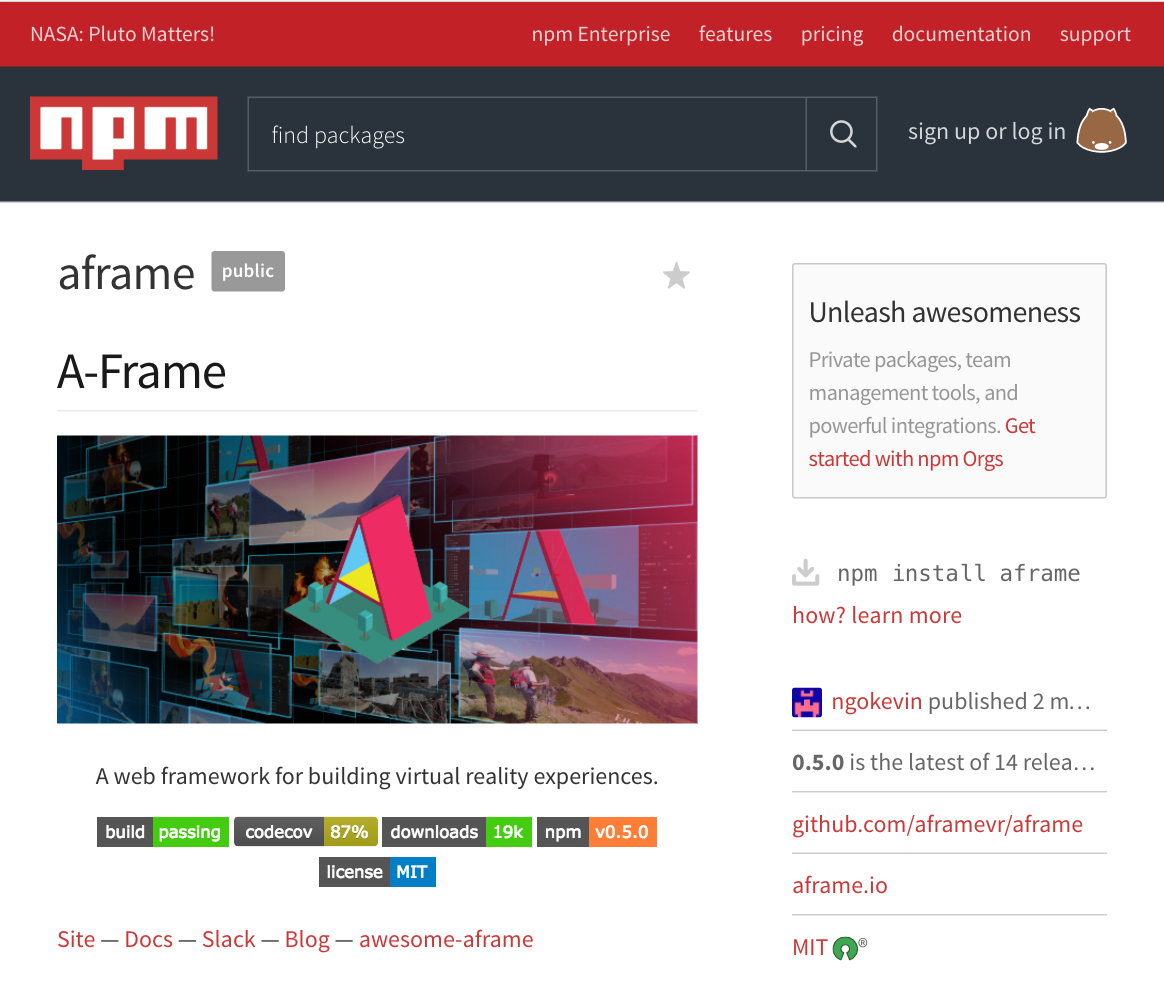
\includegraphics[width=0.9\textwidth]{npm-aframe}
\caption{Detail page of JavaScript package in NPM registry with the script to install highlighted.}
\label{r:61}
\end{figure}

To save a package into \texttt{package.json} file as a dependency, \texttt{--save} option has to be added to \texttt{npm install} command. To save it as a development dependency (only used for local development, doesn't get included in final build), we need to add \texttt{--save-dev} option instead. Packages with their respective version tag will be added to \texttt{package.json} file into specific location:

\begin{lstlisting}
"devDependencies": {
  "babel-cli": "^6.24.1",
  // ...
},
"dependencies": {
  "aframe": "^0.5.0",
  // ...
}
\end{lstlisting}

The list of used packages is included in System Manual.

\subsection{NPM scripts}
All of development, testing, bundling and deployment tasks are automated with \texttt{NPM scripts} defined in \texttt{package.json}.

\begin{lstlisting}
"scripts": {
  "start": "node server",
  "test": "jest",
  "test:watch": "npm test -- --watch",
  "coverage": "npm test -- --coverage && opn coverage/lcov-report/index.html",
  "lint": "eslint 'src/**/*.js' webpack.config.js server.js",
  "clean": "del 'build/!(.git*|Procfile)**'",
  "build:copy": "copyfiles -u 1 public/* public/**/* build",
  "build:clean": "rimraf \"build/!(.git*|Procfile)**\"",
  "prebuild": "npm run build:clean && npm run build:copy",
  "build": "cross-env NODE_ENV=production webpack"
},
\end{lstlisting}

\begin{itemize}
\item{"start" - Starts the development server.}
\item{"test" - Initialize Jest test runner that searches for all files that have \texttt{*.test.js} or \texttt{*.spec.js} in their file name and triggers all tests.}
\item{"test:watch" - Test runner will keep watching for file changes and will restart tests after every change.}
\item{"coverage" - Generates detailed test coverage report.}
\item{"lint" - Runs eslint for static code analysis testing according to preconfigured eslint rules in \texttt{.eslintrc}.}
\item{"clean" - Deletes the \texttt{/build} folder.}
\item{"build:copy" - Copies folders and files from \texttt{/public} into \texttt{/build}.}
\item{"build:clean" - Similar to "clean" command.}
\item{"prebuild" - Chain of NPM scripts that will be executed before actual "build" script.}
\item{"build" - Production-ready build that can be deployed to server.}
\end{itemize}

\subsection{Project structure}

\begin{figure}[ht!]
\centering
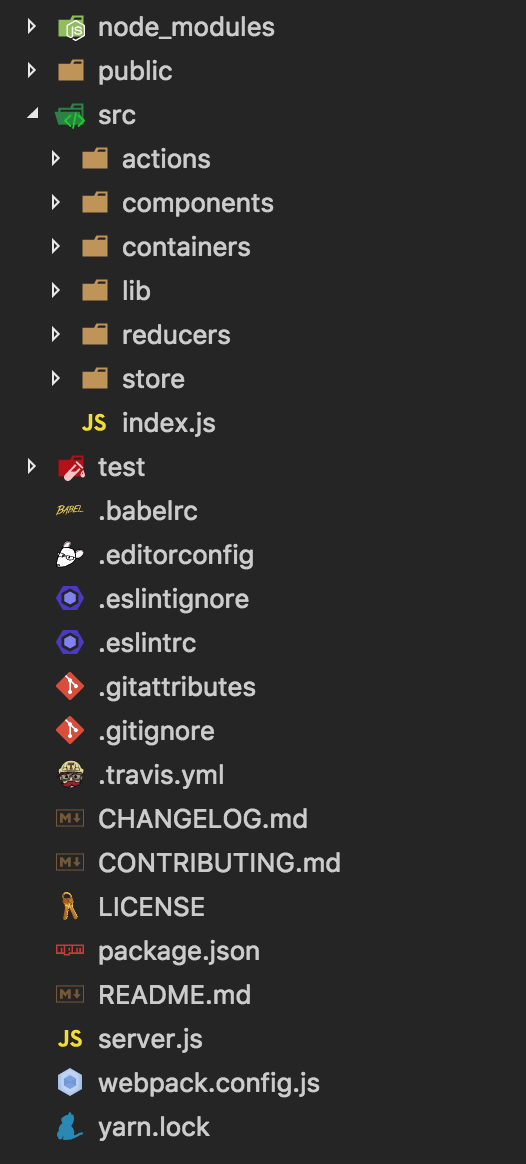
\includegraphics[width=0.3\textwidth]{folder-structure}
\caption{Project folder structure}
\label{r:62}
\end{figure}


\subsection{Webpack configuration}
Webpack is used as a tool to build JavaScript modules in MathworldVR application. It simplifies development workflow by quickly constructing a dependency graph of JavaScript application and bundling them in the right order. Our webpack configuration is defined in \texttt{webpack.config.js} and includes optimisations to the code like minification, obfuscation or splitting vendor/CSS/JavaScript code for production build. It also includes the configuration of Babel transpiler, which transpiles ES6/ES7 code to ES5, supported by all modern browsers.

\subsection{Webpack development server}
Development server configuration is defined in \texttt{server.js}. To start the server, \texttt{npm start} command is used from command line.  To properly serve the application

\begin{lstlisting}
const ip = '127.0.0.1';
const port = 3000;

new WebpackDevServer(webpack(config), {
  publicPath: '/',
  hot: true,
  host: ip,
  stats: false,
  historyApiFallback: true,
  contentBase: 'public',
}).listen(port, ip, (err) => {
  if (err) {
    return console.log(err);
  }

  console.log(`Listening at http://${ip}:${port}`);
});
\end{lstlisting}

\begin{figure}[ht!]
\centering
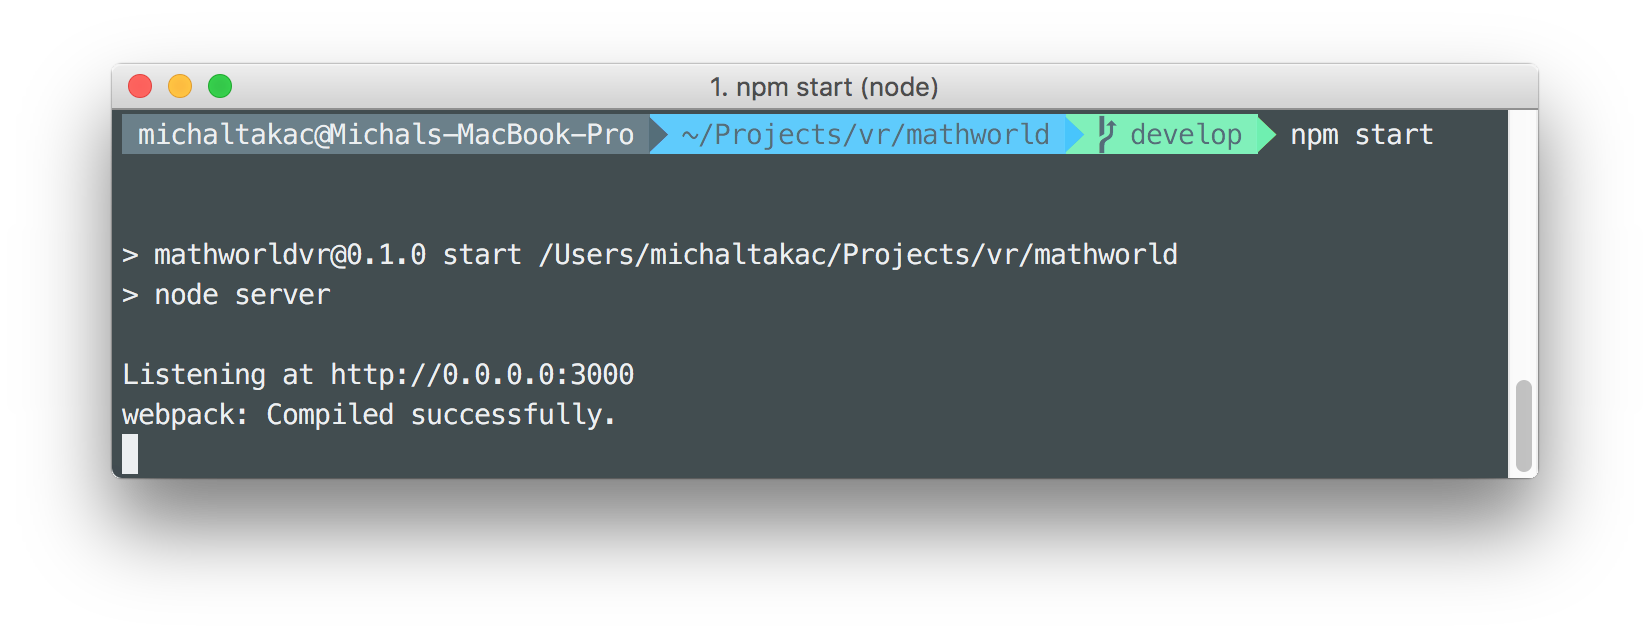
\includegraphics[width=0.6\textwidth]{npm-start}
\caption{Development server is running.}
\label{r:63}
\end{figure}

\subsection{Setting up Redux for application state management}
\begin{itemize}
\item{Actions}
\item{Reducers}
\item{Store}
\end{itemize}

\subsubsection{Initial state}
In Redux, all the application state is stored as a single object. It's a good idea to think of its shape before writing any code.

\subsubsection{Actions}
Actions are payloads of information that send data from your application to your store. They are the only source of information for the store. You send them to the store using store.dispatch().

Actions are plain JavaScript objects. Actions must have a type property that indicates the type of action being performed. Types should typically be defined as string constants.

\subsubsection{Action creators}
Action creators are functions that create actions. In Redux, action creators return an action. It makes them portable and easy to test.


\begin{lstlisting}
export const calculatorWriteText = (text) => ({
    type: CALCULATOR_WRITE_TEXT,
    text
})

export const calculatorBackspace = () => ({
    type: CALCULATOR_BACKSPACE
})

export const calculatorClearText = () => ({
    type: CALCULATOR_CLEAR_TEXT
})
\end{lstlisting}


\begin{lstlisting}
export const functionBoxSetPosition = (position) => ({
    type: FUNCTION_BOX_SET_POSITION,
    position
})
\end{lstlisting}


\begin{lstlisting}
export const parametricFunctionSetEquation = (equation) => ({
    type: PARAMETRIC_FUNCTION_SET_EQUATION,
    equation
})
\end{lstlisting}


\begin{lstlisting}
export const settingsSetXMin = (xMin) => ({
    type: SETTINGS_SET_X_MIN,
    xMin
})

export const settingsSetYMin = (yMin) => ({
    type: SETTINGS_SET_Y_MIN,
    yMin
})

export const settingsSetZMin = (zMin) => ({
    type: SETTINGS_SET_Z_MIN,
    zMin
})

export const settingsSetXMax = (xMax) => ({
    type: SETTINGS_SET_X_MAX,
    xMax
})

export const settingsSetYMax = (yMax) => ({
    type: SETTINGS_SET_Y_MAX,
    yMax
})

export const settingsSetZMax = (zMax) => ({
    type: SETTINGS_SET_Z_MAX,
    zMax
})

export const settingsSetSegments = (segments) => ({
    type: SETTINGS_SET_SEGMENTS,
    segments
})

export const settingsSetFunctionColor = (functionColor) => ({
    type: SETTINGS_SET_FUNCTION_COLOR,
    functionColor
})
\end{lstlisting}


\begin{lstlisting}
export const uiAttentionboxToggle = () => ({
    type: UI_ATTENTIONBOX_TOGGLE
})
\end{lstlisting}


\begin{lstlisting}
export const userSetPosition = (position) => ({
    type: USER_SET_POSITION,
    position
})
\end{lstlisting}

\subsubsection{Reducers}
Actions describe the fact that something happened, but don't specify how the application's state changes in response. This is the job of reducers.

The reducer is a pure function that takes the previous state and an action, and returns the next state.


\begin{lstlisting}
(previousState, action) => newState
\end{lstlisting}

It's called a reducer because it's the type of function you would pass to Array.prototype.reduce(reducer, initialValue). It's very important that the reducer stays pure. Things you should never do inside a reducer:

\begin{itemize}
\item{Mutate its arguments.}
\item{Perform side effects like API calls and routing transitions.}
\item{Call non-pure functions, e.g. Date.now() or Math.random().}
\end{itemize}

Reducer must be pure. Given the same arguments, it should calculate the next state and return it. No surprises, side effects, API calls or mutations, just a calculation.


\begin{lstlisting}[caption={\textsl{functionBox} reducer.},captionpos=b]
export default (state = initialState, action) => {
  switch (action.type) {
    case ActionTypes.FUNCTION_BOX_SET_POSITION:
      return { ...state, position: action.position }
    default: return state
  }
}
\end{lstlisting}

parametricFunction reducer:


\begin{lstlisting}
export default (state = initialState, action) => {
  switch (action.type) {
    case ActionTypes.PARAMETRIC_FUNCTION_SET_EQUATION:
      return { ...state, equation: action.equation }
    default: return state
  }
}
\end{lstlisting}

settings reducer:


\begin{lstlisting}
export default (state = initialState, action) => {
  switch (action.type) {
    case ActionTypes.SETTINGS_SET_X_MIN:
      return { ...state, xMin: action.xMin }
    case ActionTypes.SETTINGS_SET_Y_MIN:
      return { ...state, yMin: action.yMin }
    case ActionTypes.SETTINGS_SET_Z_MIN:
      return { ...state, zMin: action.zMin }
    case ActionTypes.SETTINGS_SET_X_MAX:
      return { ...state, xMax: action.xMax }
    case ActionTypes.SETTINGS_SET_Y_MAX:
      return { ...state, yMax: action.yMax }
    case ActionTypes.SETTINGS_SET_Z_MAX:
      return { ...state, zMax: action.zMax }
    case ActionTypes.SETTINGS_SET_Z_MAX:
      return { ...state, zMax: action.zMax }
    case ActionTypes.SETTINGS_SET_SEGMENTS:
      return { ...state, segments: action.segments }
    case ActionTypes.SETTINGS_SET_FUNCTION_COLOR:
      return { ...state, functionColor: action.functionColor }
    default: return state
  }
}
\end{lstlisting}

ui reducer:


\begin{lstlisting}
export default (state = initialState, action) => {
  switch (action.type) {
    case ActionTypes.UI_ATTENTIONBOX_TOGGLE:
      return { ...state, attentionBoxVisible: !state.attentionBoxVisible }
    default: return state
  }
}
\end{lstlisting}

user reducer:


\begin{lstlisting}
export default (state = initialState, action) => {
  switch (action.type) {
    case ActionTypes.USER_SET_POSITION:
      return { ...state, position: action.position }
    default: return state
  }
}
\end{lstlisting}
---

Note that:

\begin{itemize}
\item{We don't mutate the state. We create a copy with ES6 spread operator "...".}
\item{We return the previous state in the default case. It's important to return the previous state for any unknown action.}
\end{itemize}

Then we join all reducers into one, root reducer which we export from index.js:


\begin{lstlisting}
import { combineReducers } from 'redux'
import calculator from './calculator'
import functionBox from './functionBox'
import parametricFunction from './parametricFunction'
import settings from './settings'
import ui from './ui'

const rootReducer = combineReducers({
  calculator,
  functionBox,
  parametricFunction,
  settings,
  ui
})

export default rootReducer
\end{lstlisting}

combineReducers() generates a function that calls our reducers with the slices of state selected according to their keys, and combining their results into a single object again.

\subsubsection{Store}
The Store is the object that brings actions and reducers together. The store has the following responsibilities:

\begin{itemize}
\item{Holds application state.}
\item{Allows access to state via getState().}
\item{Allows state to be updated via dispatch(action).}
\item{Registers listeners via subscribe(listener).}
\item{Handles unregistering of listeners via the function returned by subscribe(listener).}
\end{itemize}

It's important to note that Redux applications only have a single store. When we want to split the data handling logic, we'll use reducer composition instead of multiple stores.

Redux Store used in development:


\begin{lstlisting}
import { createStore, applyMiddleware, compose } from 'redux'
import thunk from 'redux-thunk'
import createLogger from 'redux-logger'
import rootReducer from '../reducers'

const logger = createLogger({
  collapsed: true,
  duration: true,
})

const configureStore = initialState => {
  const hasWindow = typeof window !== 'undefined'

  const store = createStore(
    rootReducer,
    initialState,
    compose(
      applyMiddleware(thunk, logger),
      hasWindow && window.devToolsExtension ? window.devToolsExtension() : f => f
    )
  )

  if (module.hot) {
    // Enable Webpack hot module replacement for reducers
    module.hot.accept('../reducers', () => {
      const nextRootReducer = require('../reducers').default
      store.replaceReducer(nextRootReducer)
    })
  }

  return store
}

export default configureStore
\end{lstlisting}

Redux Store used in production:


\begin{lstlisting}
import { createStore, applyMiddleware } from 'redux'
import thunk from 'redux-thunk'
import rootReducer from '../reducers'

const configureStore = initialState => createStore(
  rootReducer,
  initialState,
  applyMiddleware(thunk)
)

export default configureStore
\end{lstlisting}

We'll also create additional configureStore.js file in which we'll iimplement conditional switching between Store for development and production according to NODE_ENV variable used for distinguishing between different environments:


\begin{lstlisting}
if (process.env.NODE_ENV === 'production') {
  module.exports = require('./configureStore.prod')
} else {
  module.exports = require('./configureStore.dev')
}
\end{lstlisting}

\subsection{A-Frame scene}


\begin{lstlisting}
export default class VRScene extends React.Component {
  render() {
    return (
      <a-scene>
        {this.props.children}
      </a-scene>
    )
  }
}
\end{lstlisting}

We need to import additional A-Frame-specific libraries at the start of VRScene file:


\begin{lstlisting}
// A-frame Components by community
import 'aframe'
import 'aframe-teleport-controls'
import 'super-hands'
import physics from 'aframe-physics-system'

// Libraries used by MathworldVR (Three.js, A-Frame, etc.)
import 'lib'
\end{lstlisting}

Here, we're loading aframe-physics-system which has specific initialization requirement - we need to call a function physics.registerAll() from within our scene after it's loaded. That means we need to put it inside componentWillMount function, which is React's standard lifecycle method:


\begin{lstlisting}
componentWillMount() {
  // Initialize aframe-physics-system
  physics.registerAll()
}
\end{lstlisting}

To use aframe-physics-system, we add physics="gravity: 0" to <a-scene>:


\begin{lstlisting}
<a-scene physics="gravity: 0">
  {this.props.children}
</a-scene>
\end{lstlisting}

\subsection{Camera component}
Camera component is implementing the \texttt{camera} from A-Frame API which is an abstraction over creation of a new \texttt{THREE.PerspectiveCamera} instance. Any additional properties are then passed into the main entity. \texttt{Camera} component is defined in \texttt{src/components/Camera/index.js}.

\begin{lstlisting}[caption={\textsl{Camera} component code.},captionpos=b]
import React from 'react'
import { Entity } from 'aframe-react'

const Camera = (props) => {
  return (
    <Entity camera="" {...props} />
  )
}

export default Camera
\end{lstlisting}

\subsection{Sky component}
Sky component is implementing the \texttt{geometry} and \texttt{material} from A-Frame API. It's used to achieve the feeling of a sky around the user. \texttt{geometry.primitive} property is set to \texttt{'sphere'} with \texttt{geometry.radius} of 30 meters and \texttt{sky.jpg} texture prepared for a 360-degree image viewer is added to \texttt{material.src} property, pointing to an URL where image is stored. Any additional properties are then passed into the main entity. \texttt{Sky} component is defined in \texttt{src/components/Sky/index.js}.

\begin{lstlisting}[caption={\textsl{Sky} component code.},captionpos=b]
import React from 'react'
import { Entity } from 'aframe-react'

const Sky = (props) => {
  return (
    <Entity
      geometry={{ primitive: 'sphere', radius: 30, phiLength: 360, phiStart: 0, thetaLength: 90 }}
      material={{ shader: 'flat', src: 'url(sky.jpg)', side: 'back', height: 2048, width: 2048 }}
      {...props}
    />
  )
}

export default Sky
\end{lstlisting}

\subsection{Plane component}
Plane component is implementing the \texttt{geometry} and \texttt{material} from A-Frame API. It's used as a floor under the user. \texttt{geometry.primitive} property is set to \texttt{'circle'} with \texttt{geometry.radius} of 12 meters and \texttt{floor.jpg} texture is added to \texttt{material.src} property, pointing to an URL where image is stored. Main entity is rotated 90-degrees around the X-axis. To accept light from Lights component, \texttt{material.shader} property is set to \texttt{'flat'}. Any additional properties are then passed into the main entity. \texttt{Plane} component is defined in \texttt{src/components/Plane/index.js}.

\begin{lstlisting}[caption={\textsl{Plane} component code.},captionpos=b]
import React from 'react'
import { Entity } from 'aframe-react'

const Plane = (props) => {
  return (
    <Entity
      geometry={{ primitive: 'circle', radius: 12 }}
      material={{ src: 'url(floor.jpg)', shader: 'flat', roughness: 0 }}
      rotation="-90 0 0"
      static-body
      {...props}
    />
  )
}

export default Plane
\end{lstlisting}

\subsection{Lights component}
\texttt{Lights} component is implementing the \texttt{light} from A-Frame API. It's used for lighting up the scene and main points of interest, such as FunctionBox, Calculator and SettingsPanel components. MathworldVR uses two types of light - \texttt{'point'} and \texttt{'hemisphere'}, grouped into single component. Light intensity is set with \texttt{intensity} property. \texttt{Lights} component is defined in \texttt{src/components/Lights/index.js}.

\begin{lstlisting}[caption={\textsl{Lights} component code.},captionpos=b]
import React from 'react'
import { Entity } from 'aframe-react'

const Lights = (props) => {
  return (
    <Entity {...props}>
      <Entity light={{ type: 'point', color: '#fff', intensity: 0.6 }} position={{ x: 3, y: 10, z: 1 }} />
      <Entity light={{ type: 'point', color: '#fff', intensity: 0.2 }} position={{ x: -3, y: -10, z: 1 }} />
      <Entity light={{ type: 'hemisphere,', groundColor: '#888', intensity: 0.8 }} />
    </Entity>
  )
}

export default Lights
\end{lstlisting}

\subsection{Text component}

\subsection{CalcButton component}

\subsection{Calculator component}
\subsubsection{Action types}
Calculator action types are defined in \texttt{src/actions/index.js} as string constants and exported individually to ensure they can be imported in other files and also tested.

\begin{lstlisting}[caption={\texttt{calculator} action types.},captionpos=b]
export const CALCULATOR_WRITE_TEXT = 'CALCULATOR_WRITE_TEXT'
export const CALCULATOR_BACKSPACE = 'CALCULATOR_BACKSPACE'
export const CALCULATOR_CLEAR_TEXT = 'CALCULATOR_CLEAR_TEXT'
\end{lstlisting}

\subsubsection{Action creators}
Calculator's action creators are pure functions that return payloads of information about type of \texttt{CALCULATOR} action being dispatched and, if needed, also the data we want to send to Redux store. They are defined in \texttt{src/actions/index.js}

\begin{lstlisting}[caption={Action for writing text to calculator display.},captionpos=b]
export const calculatorWriteText = (text) => ({
    type: CALCULATOR_WRITE_TEXT,
    text
})
\end{lstlisting}

\begin{lstlisting}[caption={Action to remove character from calculator display.},captionpos=b]
export const calculatorBackspace = () => ({
    type: CALCULATOR_BACKSPACE
})
\end{lstlisting}

\begin{lstlisting}[caption={Action to completely clear the calculator display.},captionpos=b]
export const calculatorClearText = () => ({
    type: CALCULATOR_CLEAR_TEXT
})
\end{lstlisting}

\subsubsection{Initial state}
Calculator component's initial state is defined in \texttt{src/reducers/calculator/index.js} as a \texttt{initialState} object.

\begin{lstlisting}[caption={Initial state of a \textsl{calculator}.},captionpos=b]
const initialState = {
  displayText: 'x^2 + y^2',
}
\end{lstlisting}

\subsubsection{Reducer function}
Reducer function for \texttt{Calculator} component is defined in \texttt{src/reducers/calculator/index.js}. From this file it's exported as a default function that takes state (with initialState as a default value) and action as its arguments and returns new state according to \texttt{CALCULATOR} actions. Possible \texttt{ActionTypes} are conditionally checked with JavaScript's \texttt{switch} statement for a better code readability.

\begin{lstlisting}[caption={Addition of text to \texttt{state.calculator.displayText} when action of type \texttt{CALCULATOR_WRITE_TEXT} is dispatched.},captionpos=b]
export default (state = initialState, action) => {
  switch (action.type) {
    // ...
    case ActionTypes.CALCULATOR_WRITE_TEXT:
      return { ...state, displayText: `${state.displayText}${action.text}` }
   // ...
    default: return state
  }
}
\end{lstlisting}

\begin{lstlisting}[caption={Remove one character from  \texttt{state.calculator.displayText} when action of type \texttt{CALCULATOR_BACKSPACE} is dispatched.},captionpos=b]
export default (state = initialState, action) => {
  switch (action.type) {
    // ...
    case ActionTypes.CALCULATOR_BACKSPACE:
      return { ...state, displayText: state.displayText.slice(0, -1) }
   // ...
    default: return state
  }
}
\end{lstlisting}

\begin{lstlisting}[caption={Clear the \texttt{state.calculator.displayText} when action of type \texttt{CALCULATOR_CLEAR_TEXT} is dispatched.},captionpos=b]
export default (state = initialState, action) => {
  switch (action.type) {
    // ...
    case ActionTypes.CALCULATOR_CLEAR_TEXT:
      return { ...state, displayText: '' }
   // ...
    default: return state
  }
}
\end{lstlisting}

\subsubsection{Higher-order component}
State and actions that Calculator component needs to function properly are mapped to properties in Calculator container, also called "higher-order component", because it's "aware" of application's state that is mapped into it. Code for Calculator higher-order component creation is defined in \texttt{src/containers/Calculator/index.js}.

\begin{lstlisting}[caption={Function to map \texttt{calculator} state to component properties.},captionpos=b]
const mapStateToProps = (state) => ({
  displayText: state.calculator.displayText,
})
\end{lstlisting}

\begin{lstlisting}[caption={Function to map dispatchable \texttt{calculator} action creators to component properties.},captionpos=b]
const mapDispatchToProps = (dispatch) => ({
  writeText: (text) => dispatch(calculatorWriteText(text)),
  backspace: () => dispatch(calculatorBackspace()),
  clearText: () => dispatch(calculatorClearText()),
  updateEquation: (equation) => dispatch(parametricFunctionSetEquation(equation)),
})
\end{lstlisting}

\begin{lstlisting}[caption={Creation of \texttt{Calculator} higher-order component.},captionpos=b]
import { connect } from 'react-redux'
import { Calculator } from 'components'
// ...
export default connect(mapStateToProps, mapDispatchToProps)(Calculator)
\end{lstlisting}

\subsubsection{Presentational component}
Presentational Calculator component is implementing the \texttt{geometry} and \texttt{material} from A-Frame API. It's shape is determined by \texttt{geometry.primitive} which is set to \texttt{'box'} with width of \texttt{0.88} meters, height of \texttt{0.65} meters and depth of \texttt{0.01} meters. By default it's not moveable to ensure its position central to the MathworldVR experience. Properties passed into the component as function attributes includes state and dispatchable action that was mapped in it's higher-order component. \texttt{Calculator} code is defined in \texttt{src/components/Calculator/index.js}. Code preview displayed here doesn't include the CalcButton components, but they're utilizing the \texttt{writeText}, \texttt{backspace} and \texttt{clearText} actions. They will be explained in next section.

\begin{lstlisting}[caption={Presentational \texttt{Calculator} component code.},captionpos=b]
const Calculator = ({ displayText, writeText, backspace, clearText, updateEquation }) => {
  return (
    <Entity
      geometry="primitive: box; width: 0.88; height: 0.65; depth: 0.01;"
      material="shader: flat; side: double; color: #8d8547;"
    >
      { /* Calculator display */ }
      <Text value={displayText} />
      
      { /* --- BUTTONS --- */ }
      { /* ... */ }
      
    </Entity>
  )
}
      
\end{lstlisting}


\subsection{CalcButton component}


\begin{lstlisting}
import React from 'react'
import PropTypes from 'prop-types'
import { Entity } from 'aframe-react'
import { Text } from 'components'

export default class CalcButton extends React.Component {
  constructor(props) {
    super(props)

    this.state = {
      depth: 0.02,
      opacity: 1,
    }

    this.startIntersection = this.startIntersection.bind(this)
    this.endIntersection = this.endIntersection.bind(this)
  }

  startIntersection() {
    const { actionToTrigger, value } = this.props
    this.setState({ depth: 0, opacity: 0.2 })
    actionToTrigger(value)
  }

  endIntersection() {
    this.setState({ depth: 0.02, opacity: 1 })
  }

  render() {
    const { id, position, width, height, buttonColor, text, textColor, textWidth } = this.props
    const { depth, opacity } = this.state
    return (
      <Entity
        id={id}
        className="interactive"
        geometry={{ primitive: 'box', height, width, depth }}
        material={{ shader: 'flat', side: 'double', color: buttonColor, opacity }}
        scale={{ x: 0.5, y: 0.5, z: 0.5 }}
        position={position}
        hoverable
        clickable
        events={{
          'hover-start': this.startIntersection,
          'hover-end': this.endIntersection,
        }}
      >
        <Text
          value={text}
          color={textColor}
          align="center"
          zOffset={0.02}
          width={textWidth}
        />
      </Entity>
    )
  }
}
\end{lstlisting}


\subsection{Adding components together}
\begin{figure}[ht!]
\centering
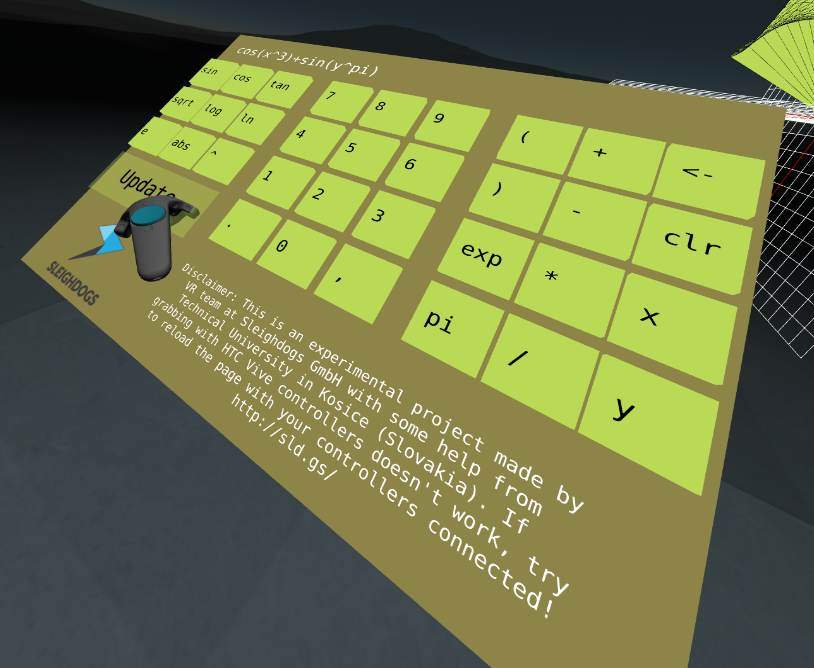
\includegraphics[width=0.6\textwidth]{calculator}
\caption{Calculator component}
\label{r:2}
\end{figure}

\subsection{ParametrizedFunction component}
\subsubsection{Extending A-Frame API with parametrizedfunction component}


\begin{lstlisting}[caption={Registering new A-Frame component \texttt{'parametricfunction'}.},captionpos=b]
AFRAME.registerComponent('parametricfunction', {
  schema: {/* ... */}, 
  init: function() {/* ... */},
  update: function() {/* ... */},
  remove: function() {/* ... */},
})
\end{lstlisting}

\begin{lstlisting}[caption={\texttt{parametricfunction} A-Frame component schema with default values.},captionpos=b]
schema: {
  equation: { type: 'string', default: '' },
  segments: { type: 'number', default: 20 },
  xMin: { type: 'number', default: -5 },
  xMax: { type: 'number', default: 5 },
  yMin: { type: 'number', default: -5 },
  yMax: { type: 'number', default: 5 },
  zMin: { type: 'number', default: -5 },
  zMax: { type: 'number', default: 5 },
  functionColor: { type: 'string', default: '#bada55' }
}
\end{lstlisting}

\begin{lstlisting}[caption={\texttt{parametricfunction} A-Frame component init function.},captionpos=b]
init: function() {
  const el = this.el;
  const canvas = el.sceneEl.canvas;
  // Wait for canvas to load.
  if (!canvas) {
    el.sceneEl.addEventListener('render-target-loaded', this.init.bind(this));
    return;
  }
}
\end{lstlisting}

\begin{lstlisting}[caption={\texttt{parametricfunction} A-Frame component init function.},captionpos=b]
var equation = 'f(x,y) = ' + this.data.equation;
var parser = math.parser();
\end{lstlisting}

\begin{lstlisting}[caption={\texttt{parametricfunction} A-Frame component init function.},captionpos=b]
try {
  parser.eval(equation);
} catch (error) {
  return;
}
\end{lstlisting}

\begin{lstlisting}[caption={\texttt{parametricfunction} A-Frame component init function.},captionpos=b]
const f1 = parser.get('f');
parser.clear();
\end{lstlisting}

\begin{lstlisting}[caption={\texttt{parametricfunction} A-Frame component init function.},captionpos=b]
this.mainMaterial = new THREE.MeshBasicMaterial( { color: this.data.functionColor, side: THREE.DoubleSide } );
this.wireframeMaterial = new THREE.MeshBasicMaterial( { color: 0x00008, wireframe: true, transparent: true } );
this.functionMaterial = [ this.mainMaterial, this.wireframeMaterial ];
\end{lstlisting}
    
\subsubsection{Action types}
ParametricFunction action types are defined in \texttt{src/actions/index.js} as string constants and exported individually to ensure they can be imported in other files and also tested.

\begin{lstlisting}[caption={\texttt{parametricFunction} action types.},captionpos=b]
export const PARAMETRIC_FUNCTION_SET_EQUATION = 'PARAMETRIC_FUNCTION_SET_EQUATION'
\end{lstlisting}

\subsubsection{Action creators}
ParametricFunction's action creators are pure functions that return payloads of information about type of \texttt{PARAMETRIC_FUNCTION} action being dispatched and, if needed, also the data we want to send to Redux store. They are defined in \texttt{src/actions/index.js}

\begin{lstlisting}[caption={Action for setting the function for 3D visualization.},captionpos=b]
export const parametricFunctionSetEquation = (equation) => ({
  type: PARAMETRIC_FUNCTION_SET_EQUATION,
  equation,
})
\end{lstlisting}

\subsubsection{Initial state}
ParametricFunction component's initial state is defined in \texttt{src/reducers/parametrizedFunction/index.js} as a \texttt{initialState} object.

\begin{lstlisting}[caption={Initial state of a \textsl{calculator}.},captionpos=b]
const initialState = {
  equation: 'x^2 + y^2',
}
\end{lstlisting}

\subsubsection{Reducer function}
Reducer function for \texttt{ParametricFunction} component is defined in \texttt{src/reducers/parametricFunction/index.js}. From this file it's exported as a default function that takes state (with initialState as a default value) and action as its arguments and returns new state according to \texttt{PARAMETRIC_FUNCTION} actions. Possible \texttt{ActionTypes} are conditionally checked with JavaScript's \texttt{switch} statement for a better code readability.

\begin{lstlisting}[caption={Update the \texttt{state.parametricFunction.equation} value with the new one from action payload when action of type \texttt{PARAMETRIC_FUNCTION_SET_EQUATION} is dispatched.},captionpos=b]
export default (state = initialState, action) => {
  switch (action.type) {
    // ...
    case ActionTypes.PARAMETRIC_FUNCTION_SET_EQUATION:
      return { ...state, equation: action.equation }
   // ...
    default: return state
  }
}
\end{lstlisting}

\subsubsection{Higher-order component}
State and actions that ParametricFunction component needs to function properly are mapped to properties in ParametricFunction container - higher-order component. Code for ParametricFunction higher-order component creation is defined in \texttt{src/containers/ParametricFunction/index.js}.

\begin{lstlisting}[caption={Function to map \texttt{parametricFunction}  and \texttt{settings} state to component properties.},captionpos=b]
const mapStateToProps = (state) => ({
  equation: state.parametricFunction.equation,
  segments: state.settings.segments,
  xMin: state.settings.xMin,
  xMax: state.settings.xMax,
  yMin: state.settings.yMin,
  yMax: state.settings.yMax,
  zMin: state.settings.zMin,
  zMax: state.settings.zMax,
  functionColor: state.settings.functionColor,
})
\end{lstlisting}

\begin{lstlisting}[caption={Creation of \texttt{ParametricFunction} higher-order component.},captionpos=b]
import { connect } from 'react-redux'
import { ParametricFunction } from 'components'
// ...
export default connect(mapStateToProps)(ParametricFunction)
\end{lstlisting}

\subsubsection{Presentational component}
Presentational ParametricFunction component is implementing the \texttt{geometry} and \texttt{material} from A-Frame API. It's shape is determined by \texttt{geometry.primitive} which is set to \texttt{'box'} with width of \texttt{0.88} meters, height of \texttt{0.65} meters and depth of \texttt{0.01} meters. By default it's not moveable to ensure its position central to the MathworldVR experience. Properties passed into the component as function attributes includes state and dispatchable action that was mapped in it's higher-order component. \texttt{Calculator} code is defined in \texttt{src/components/Calculator/index.js}. Code preview displayed here doesn't include the CalcButton components, but they're utilizing the \texttt{writeText}, \texttt{backspace} and \texttt{clearText} actions. They will be explained in next section.

\begin{lstlisting}[caption={Presentational \texttt{ParametricFunction} component code.},captionpos=b]
const ParametricFuntion = ({ equation, segments, xMin, xMax, yMin, yMax, zMin, zMax, functionColor }) => {
  return (
    <Entity
      id="function-mesh"
      parametricfunction={{
        equation,
        segments,
        xMin,
        xMax,
        yMin,
        yMax,
        zMin,
        zMax,
        functionColor,
      }}
      grid="size: 2; step: 20"
    />
  )
}
\end{lstlisting}

\subsection{SettingsPanel component}

We will register the datgui A-Frame component first. Inside the init method, we're creating the dat.guiVR instance and injecting it into the component element property:

\begin{lstlisting}
const gui = dat.GUIVR.create( this.data.name );
this.el.setObject3D('gui', gui );
this.el.gui = gui;
\end{lstlisting}

To allow VR hand controllers interactions, we'll create bindInput method that will create event listeners for triggerdown, triggerup, gripdown and gripup events:

\begin{lstlisting}
function bindInput( el, input ){
  el.addEventListener('triggerdown', function() {
    input.pressed(true);
  });
  el.addEventListener('triggerup', function() {
    input.pressed(false);
  });
  el.addEventListener('gripdown', function() {
    input.gripped(true);
  });
  el.addEventListener('gripup', function() {
    input.gripped(false);
  });
}
\end{lstlisting}

Datgui component doesn't know about the VR hand controllers yet, thus we need to add them as an input objects into dat.guiVR instance:


\begin{lstlisting}
const controllerRightEl = this.data.controllerRight;
if (controllerRightEl){
  const right = dat.GUIVR.addInputObject(controllerRightEl.object3D);
  scene.add(right);
  bindInput(controllerRightEl, right);
}

const controllerLeftEl = this.data.controllerLeft;
if (controllerLeftEl){
  const left = dat.GUIVR.addInputObject( controllerLeftEl.object3D);
  scene.add(left);
  bindInput(controllerLeftEl, left);
}
\end{lstlisting}

After the datgui component, we'll create 

\begin{figure}[ht!]
\centering
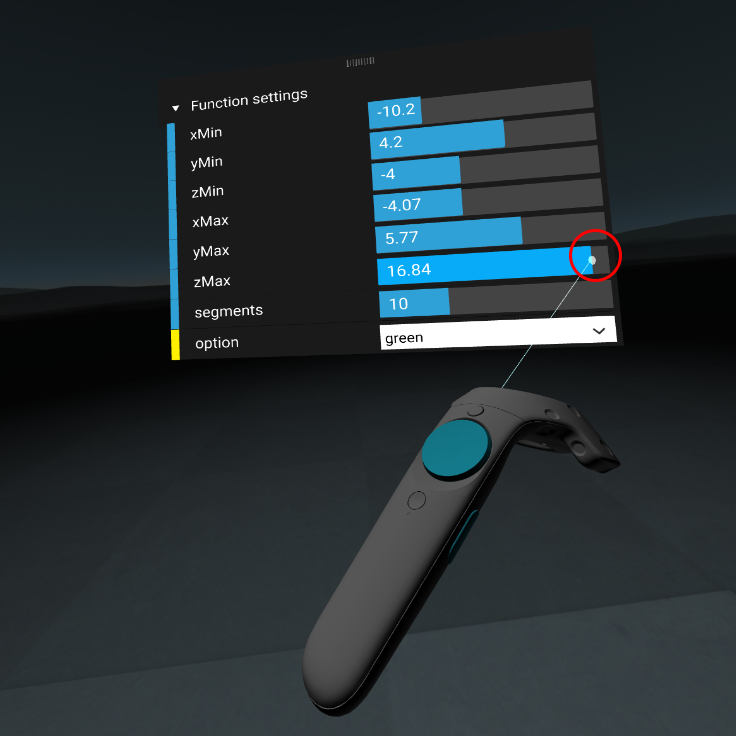
\includegraphics[width=0.6\textwidth]{function_settings}
\caption{SettingsPanel component}
\label{r:4}
\end{figure}

\subsection{Hand controller components}


\begin{lstlisting}
import React from 'react'
import { Entity } from 'aframe-react'

const RightController = (props) => {
  return (
    <Entity
      id="rightController"
      hand-controls="right"
      sphere-collider={{ objects: '.interactive', radius: 0.05 }}
      if-no-vr-headset={{ visible: false }}
      super-hands
      static-body={{ shape: 'sphere', sphereRadius: 0.05 }}
      {...props}
    />
  )
}

export default RightController
\end{lstlisting}


\begin{lstlisting}
import React from 'react'
import { Entity } from 'aframe-react'

const LeftController = (props) => {
  return (
    <Entity
      id="leftController"
      hand-controls="left"
      sphere-collider={{ objects: '.interactive', radius: 0.05 }}
      if-no-vr-headset={{ visible: false }}
      teleport-controls
      super-hands
      static-body={{ shape: 'sphere', sphereRadius: 0.05 }}
      {...props}
    />
  )
}

export default LeftController
\end{lstlisting}

\subsection{Adding components into A-Frame scene}


\begin{lstlisting}
<VRScene>
  <AttentionBox />
  <LeftController />
  <RightController />

  <FunctionBox>
    <ParametricFunction />
  </FunctionBox>

  <Calculator />

  <SettingsPanel
    name="Function settings"
    position={{ x: -0.37, y: 1.93, z: -0.34 }}
    rotation={{ x: 10, y: 30, z: 0 }}
    scale={{ x: 0.5, y: 0.5, z: 0.5 }}
  />

  <Sky />
  <Lights />
  <Plane />
</VRScene>
\end{lstlisting}

\subsection{Interactions}

\subsubsection{Grabbing}

\begin{figure}[ht!]
\centering
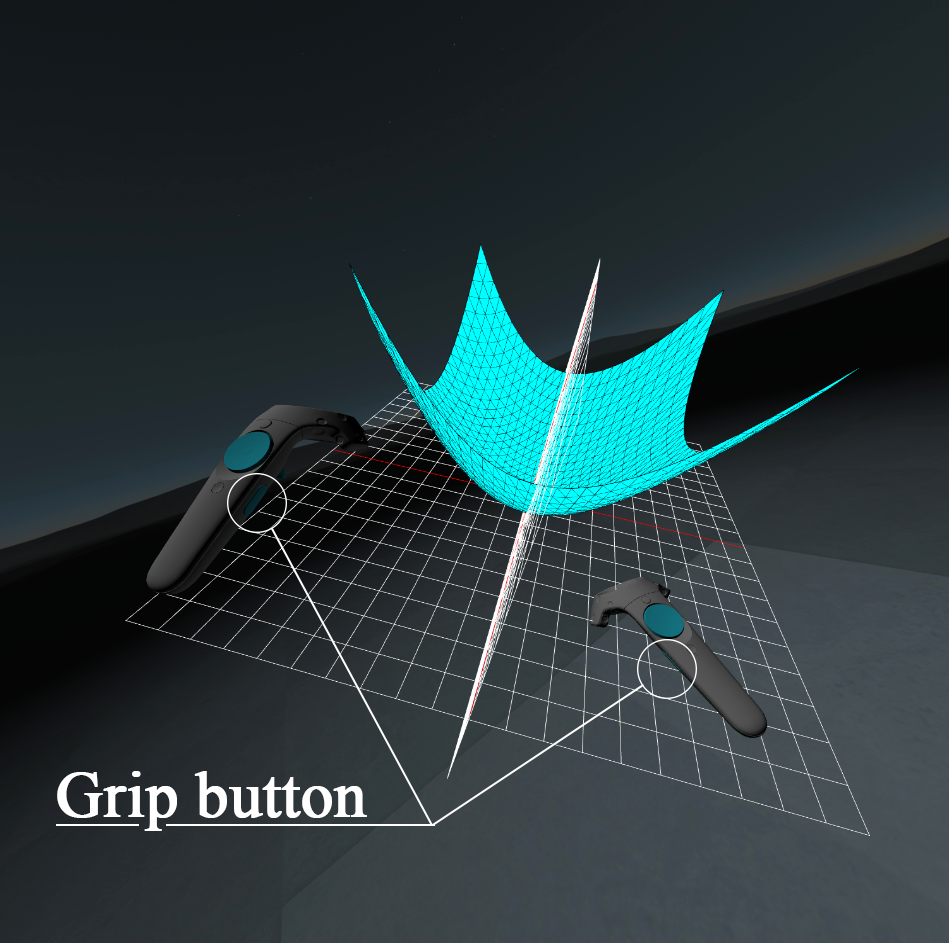
\includegraphics[width=0.6\textwidth]{grab}
\caption{Grabbing functionality}
\label{r:5}
\end{figure}

\subsubsection{Scaling}

\begin{figure}[ht!]
\centering
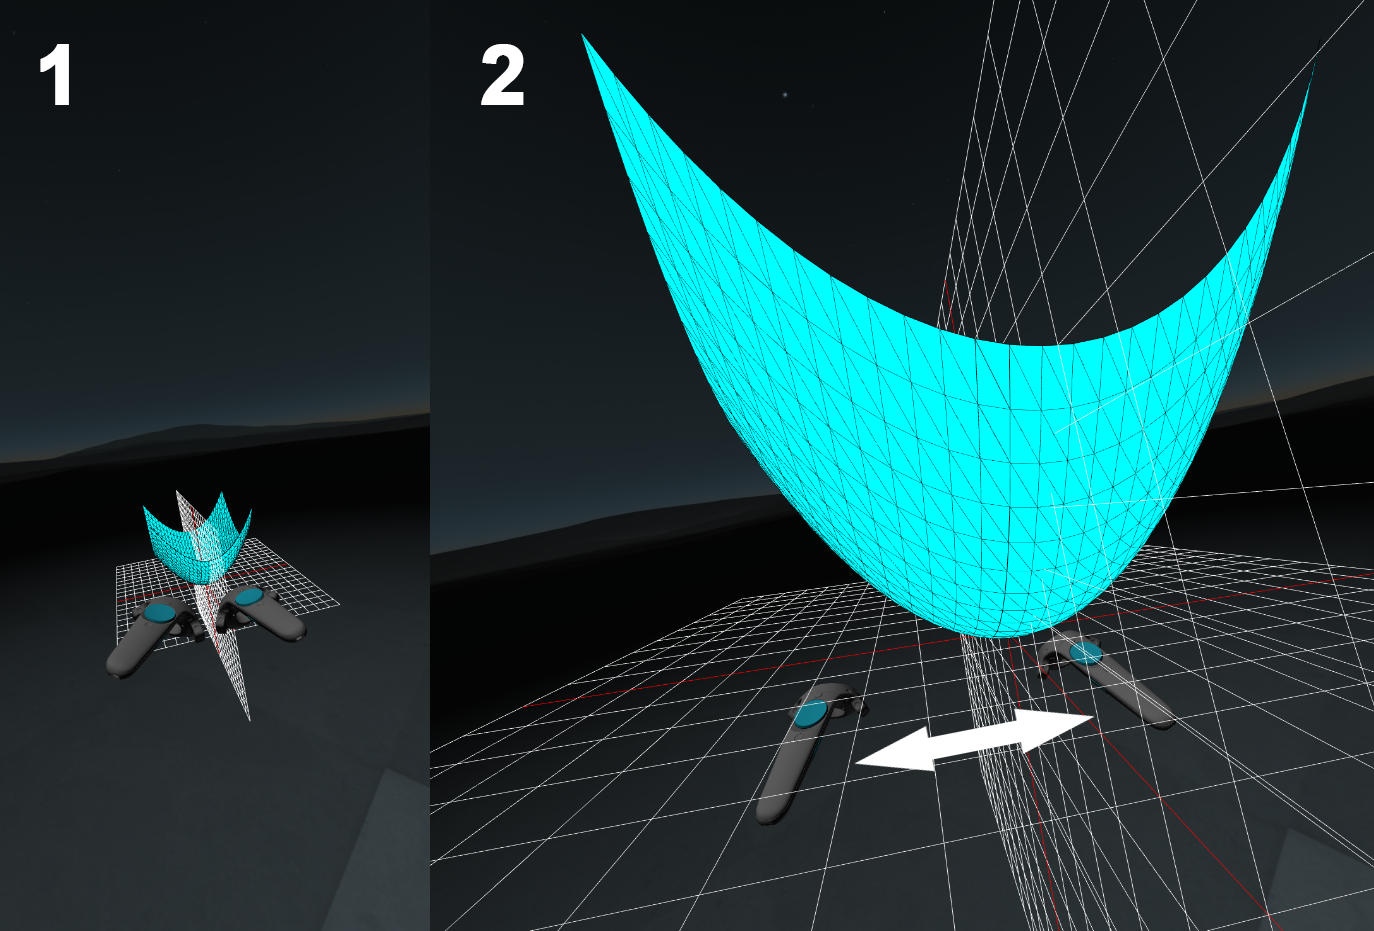
\includegraphics[width=0.6\textwidth]{scaling}
\caption{Scaling functionality}
\label{r:6}
\end{figure}

\subsection{Parsing equations with Math.js}


\subsection{AttentionBox component}


\subsection{Building and deploying the application to web hosting}


%Začnime rovnicou
%
%\begin{equation}\label{r:2}
%\frac{\ud^2y}{\ud t^2}+\frac{\ud y}{\ud t}+y =0, \qquad y(0)=1, \quad
%y\,'(0)=15.
%\end{equation}
%
%Grafický priebeh riešenia tejto rovnice vidíme na Obrázku \ref{o:2}.
%
%\begin{figure}[ht!]
%\centering
%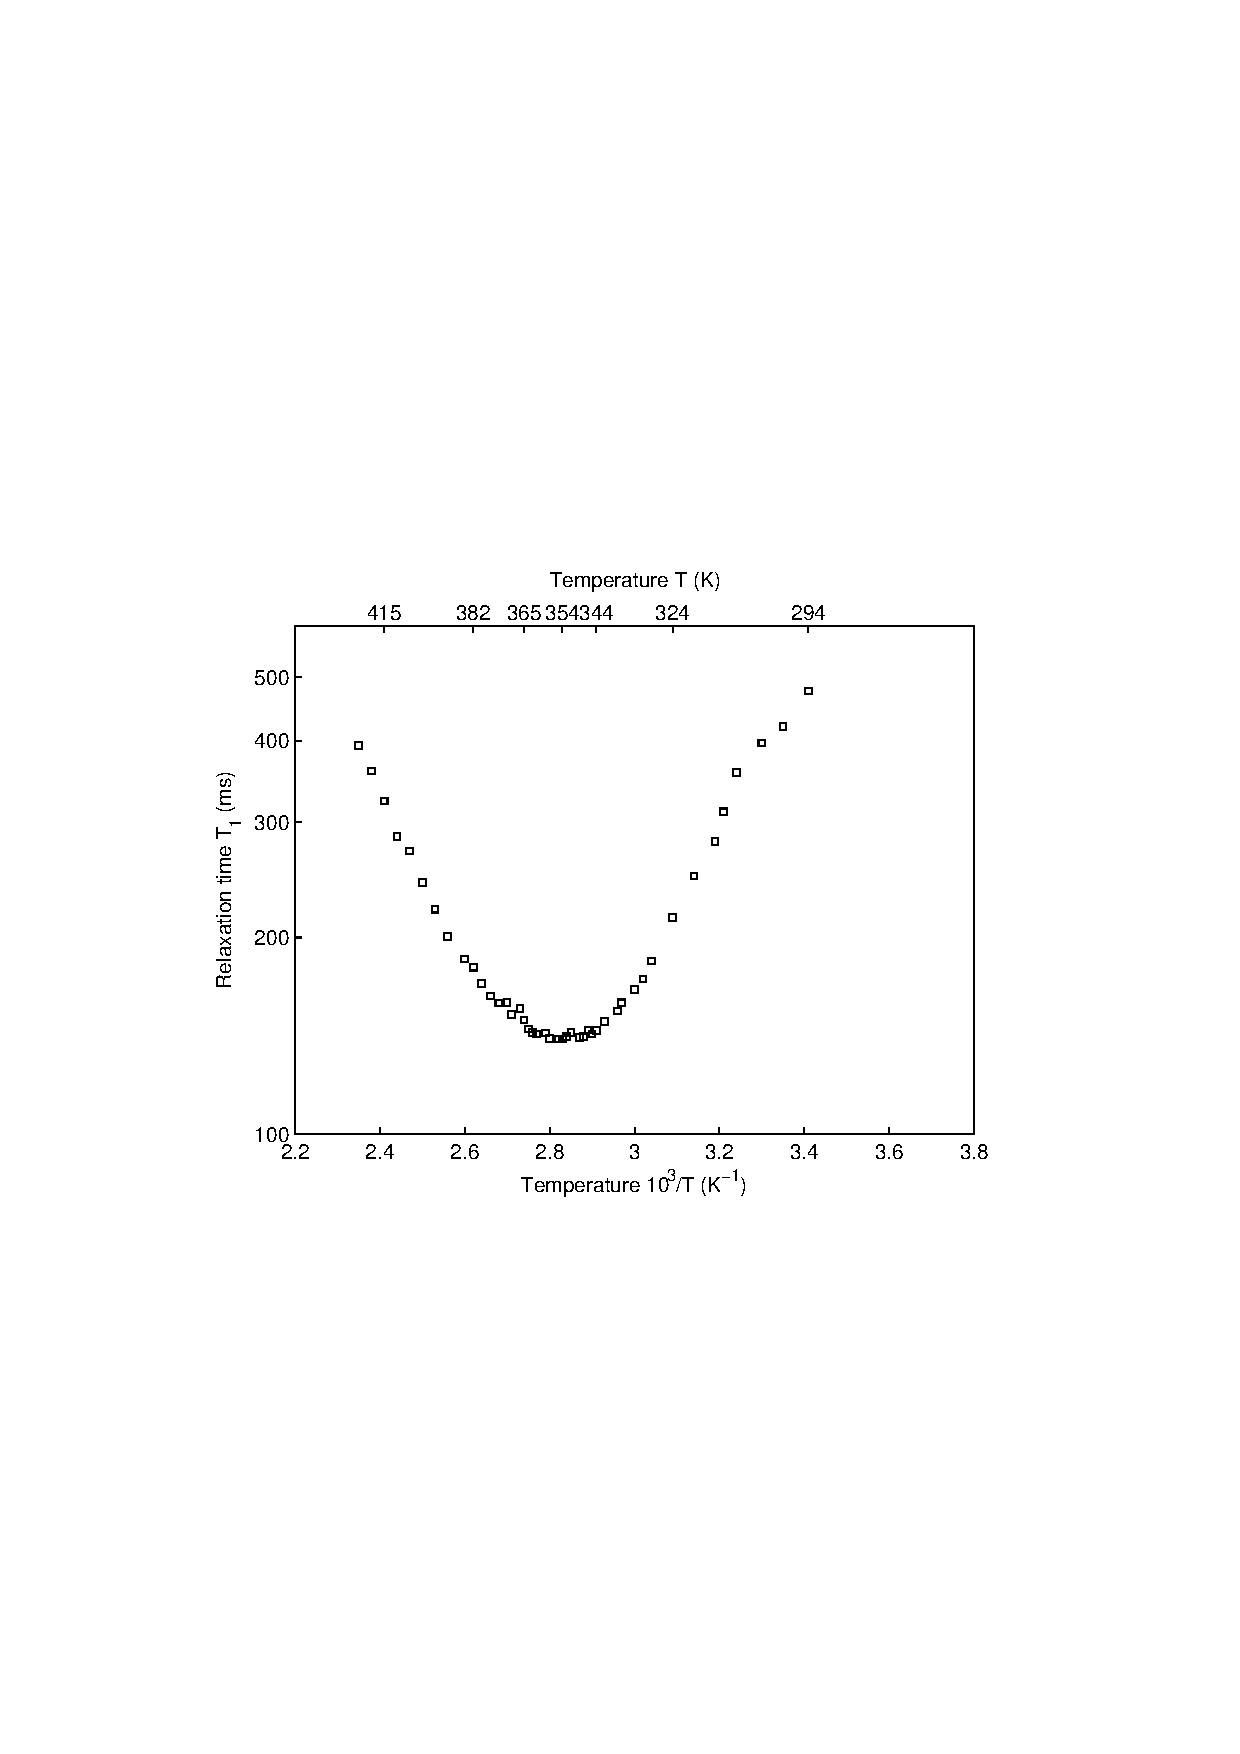
\includegraphics[width=.6\textwidth,angle=0]{relaxcas.pdf}
%\caption{Teplotná závislosť\/ spinovo-mriežkového relaxačného
%času}\label{o:3}
%\end{figure}
%
%%\tabcolsep=3pt % sirka stlpcov
%%\renewcommand{\arraystretch}{1.2} % riadkovanie
%\begin{table}[ht!]
%\centering
%\caption{Parametre získané z~meraní spinovo-mriežkových relaxačných
%časov $T_1$}\label{t:2}
%\medskip
%\newcolumntype{d}{D{,}{,}{-1}}
%\begin{tabular}{||c||d|d|d|d|d||}
%\hhline{|t:==t:==:==:t|}
%\multicolumn{1}{||c||}{}&\multicolumn{1}{c|}{PP --
%01}&\multicolumn{1}{c|}{PP -- 05}&\multicolumn{1}{c|}{PP --
%10}&\multicolumn{1}{c|}{PP -- 16}&\multicolumn{1}{c||}{PP -- 22} \\
%\hhline{|:==:==:==:|}
%C $\cdot 10^8$~(s$^{-2}$) & 10,1 & 10,0 & 11,0 & 9,2 & 8  \\
%\hhline{||-|-|-|-|-|-||}
%$\tau_0 \cdot 10^{-14}$~(s) & 2,63 & 1,44 & 0,95 & 2,21 & 10,83  \\
%\hhline{||-|-|-|-|-|-||}
%$E_{\text a}$~(kJ) & 34,26 & 8,33 & 39,76 & 37,31 & 31,86  \\
%\hhline{||-|-|-|-|-|-||}
%$T_{\min}$~(K) & 354 & 367 & 367 & 369 & 367  \\
%\hhline{||-|-|-|-|-|-||}
%$T_{1\min}$~(ms) & 141 & 160 & 157 & 175 & 181  \\
%\hhline{||-|-|-|-|-|-||}
%$\Delta M_2$~(Gs$^2$) & 5,49 & 5,66 & 5,16 & 5,09 & 5,02  \\
%\hhline{|b:==b:==:==:b|}
%\end{tabular}
%\end{table}

